%%%%%%%%%%%%%%%%%%%%%%%%%%%%%%%%%%%%%%%%%
% Beamer Presentation
% LaTeX Template
% Version 1.0 (10/11/12)
%
% This template has been downloaded from:
% http://www.LaTeXTemplates.com
%
% License:
% CC BY-NC-SA 3.0 (http://creativecommons.org/licenses/by-nc-sa/3.0/)
%
%%%%%%%%%%%%%%%%%%%%%%%%%%%%%%%%%%%%%%%%%

%----------------------------------------------------------------------------------------
%	PACKAGES AND THEMES
%----------------------------------------------------------------------------------------

\documentclass{beamer}

\mode<presentation> {

% The Beamer class comes with a number of default slide themes
% which change the colors and layouts of slides. Below this is a list
% of all the themes, uncomment each in turn to see what they look like.

%\usetheme{default}
%\usetheme{AnnArbor}
%\usetheme{Antibes}
%\usetheme{Bergen}
%\usetheme{Berkeley}
%\usetheme{Berlin}
%\usetheme{Boadilla}
%\usetheme{CambridgeUS}
%\usetheme{Copenhagen}
%\usetheme{Darmstadt}
%\usetheme{Dresden}
%\usetheme{Frankfurt}
%\usetheme{Goettingen}
%\usetheme{Hannover}
%\usetheme{Ilmenau}
%\usetheme{JuanLesPins}
%\usetheme{Luebeck}
%\usetheme{Madrid}
%\usetheme{Malmoe}
%\usetheme{Marburg}
%\usetheme{Montpellier}
%\usetheme{PaloAlto}
%\usetheme{Pittsburgh}
%\usetheme{Rochester}
%\usetheme{Singapore}
\usetheme{Szeged}
%\usetheme{Warsaw}

% As well as themes, the Beamer class has a number of color themes
% for any slide theme. Uncomment each of these in turn to see how it
% changes the colors of your current slide theme.

%\usecolortheme{albatross}
\usecolortheme{beaver}
%\usecolortheme{beetle}
%\usecolortheme{crane}
%\usecolortheme{dolphin}
%\usecolortheme{dove}
%\usecolortheme{fly}
%\usecolortheme{lily}
%\usecolortheme{orchid}
%\usecolortheme{rose}
%\usecolortheme{seagull}
%\usecolortheme{seahorse}
%\usecolortheme{whale}
%\usecolortheme{wolverine}

%\setbeamertemplate{footline} % To remove the footer line in all slides uncomment this line
%\setbeamertemplate{footline}[page number] % To replace the footer line in all slides with a simple slide count uncomment this line

%\setbeamertemplate{navigation symbols}{} % To remove the navigation symbols from the bottom of all slides uncomment this line
}

\usepackage{graphicx} % Allows including images
\usepackage{booktabs} % Allows the use of \toprule, \midrule and \bottomrule in tables
\usepackage{hyperref}
\usepackage{xcolor}

%----------------------------------------------------------------------------------------
%	TITLE PAGE
%----------------------------------------------------------------------------------------

\title[MC Rates]{Monte Carlo Rate Comparisons} % The short title appears at the bottom of every slide, the full title is only on the title page

\author{Matt Solt} % Your name
\institute[Stanford] % Your institution as it will appear on the bottom of every slide, may be shorthand to save space
{
SLAC National Accelerator Laboratory \\ % Your institution for the title page
\medskip
\textit{mrsolt@slac.stanford.edu} % Your email address
}
\date{\today} % Date, can be changed to a custom date

\begin{document}

\begin{frame}
\titlepage % Print the title page as the first slide
\end{frame}

%----------------------------------------------------------------------------------------
%	PRESENTATION SLIDES
%----------------------------------------------------------------------------------------

%------------------------------------------------
%\section{First Section} % Sections can be created in order to organize your presentation into discrete blocks, all sections and subsections are automatically printed in the table of contents as an overview of the talk
%------------------------------------------------

%\subsection{Subsection Example} % A subsection can be created just before a set of slides with a common theme to further break down your presentation into chunks

\begin{frame}
\frametitle{Introduction}
\begin{itemize}
\item MC compared
\begin{itemize}
\item MG5 tritrig
\item MG4 wabs
\item 10\% 2015 Data
\item MG5 tritrig-wab-beam
\item MG4/5 wab-beam-tri
\end{itemize}
\end{itemize}

\end{frame}

%------------------------------------------------

\begin{frame}
\frametitle{Cross Section Comparison}
\begin{itemize}
\item Tritrig is consistantly a factor of 2 greater than data for me... why?
\item Tritrig-wab-beam is consistantly a factor of 2 less than data for me... why?
\end{itemize}
\begin{figure}
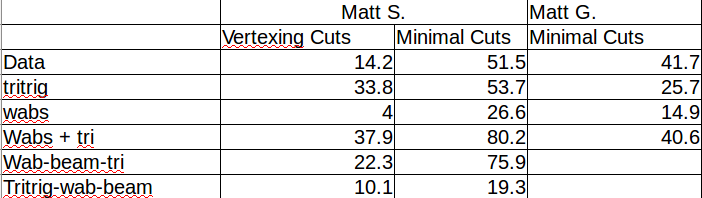
\includegraphics[width=1.0\linewidth]{figs/table2.png}
\end{figure}

\end{frame}

%------------------------------------------------

\begin{frame}
\frametitle{P Sum Comparison 1/2}
\begin{itemize}
\item Minimal cuts - $P_{track}<0.8 E_{beam}$, opposite volume, $P>0.8 E_{beam}$, and $|\Delta t_{cl}| < 2$ ns
\item Left is Matt S. Right is Matt G.
\end{itemize}
\begin{figure}
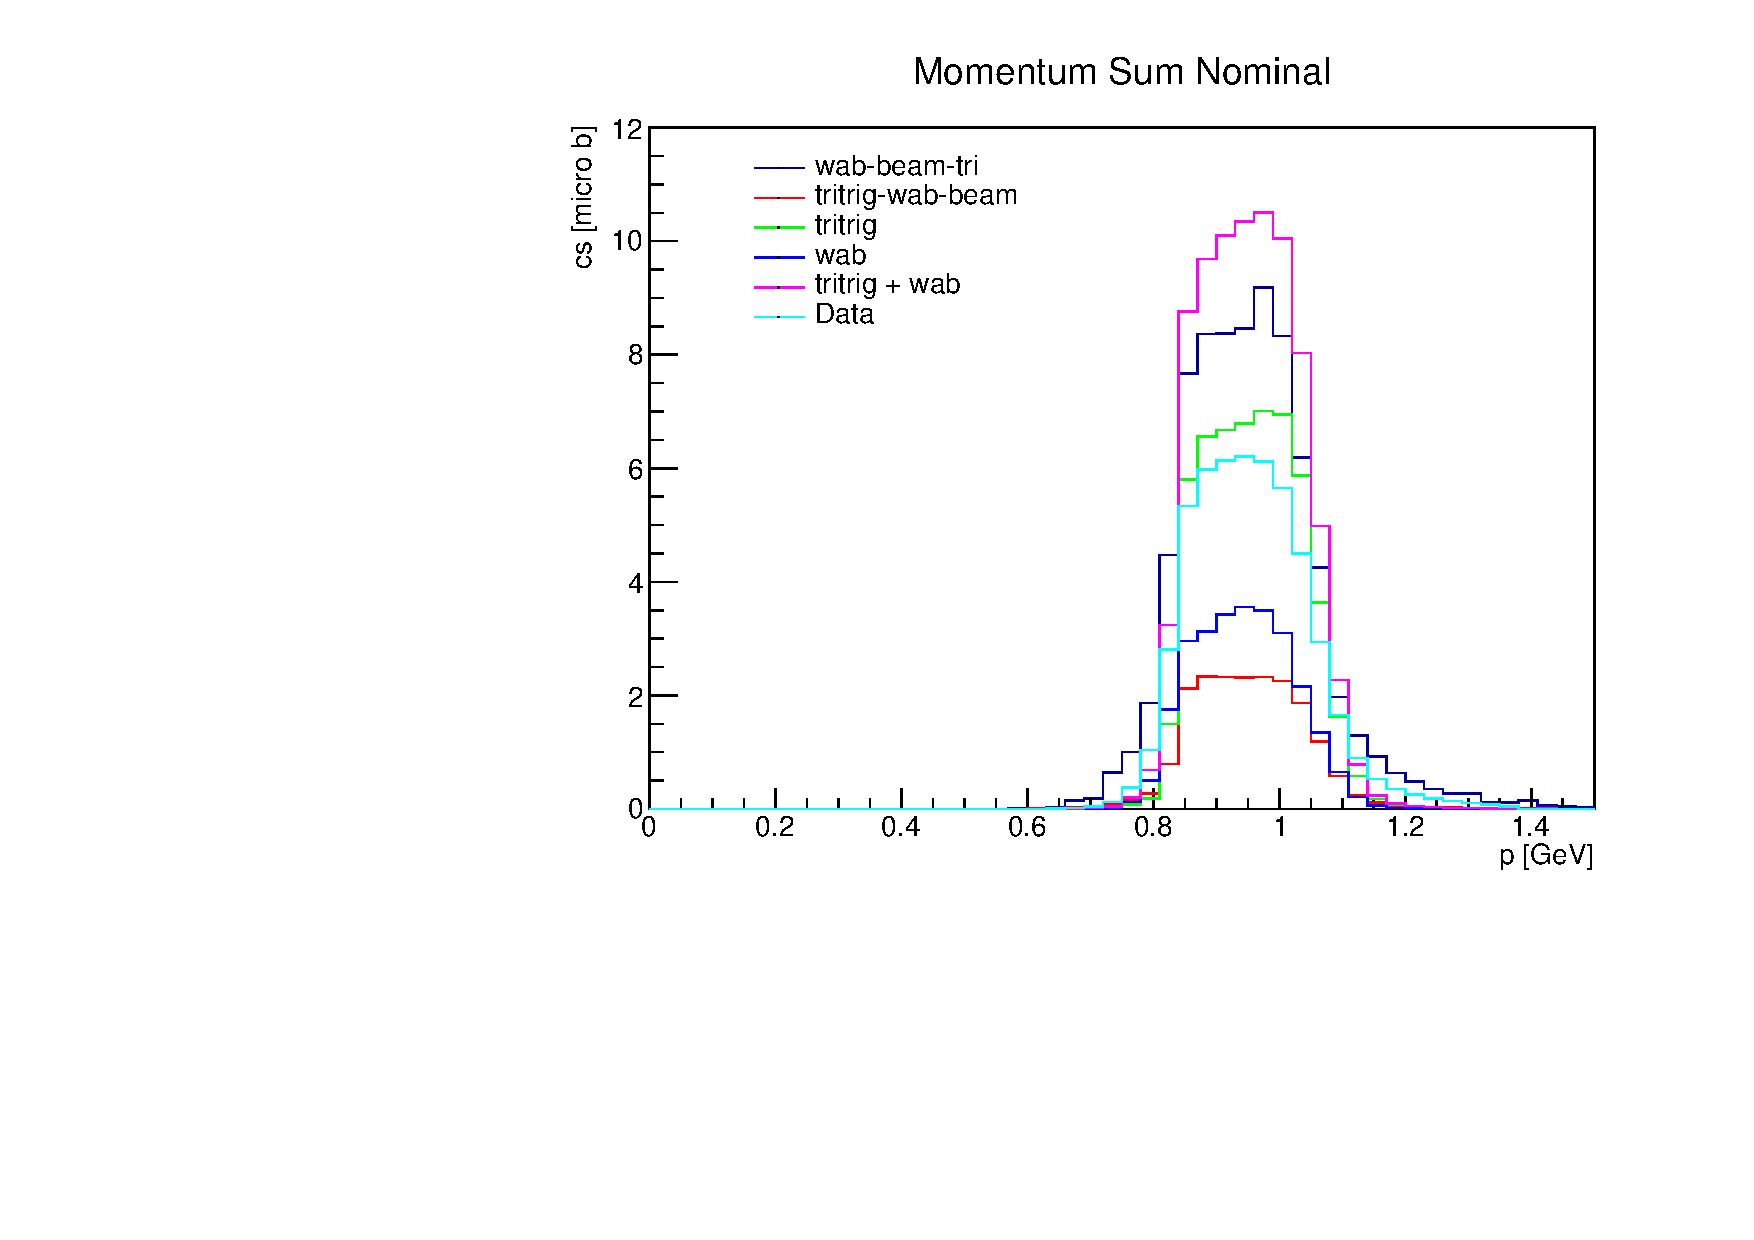
\includegraphics[width=0.55\linewidth]{figs/psum_minimal.pdf}
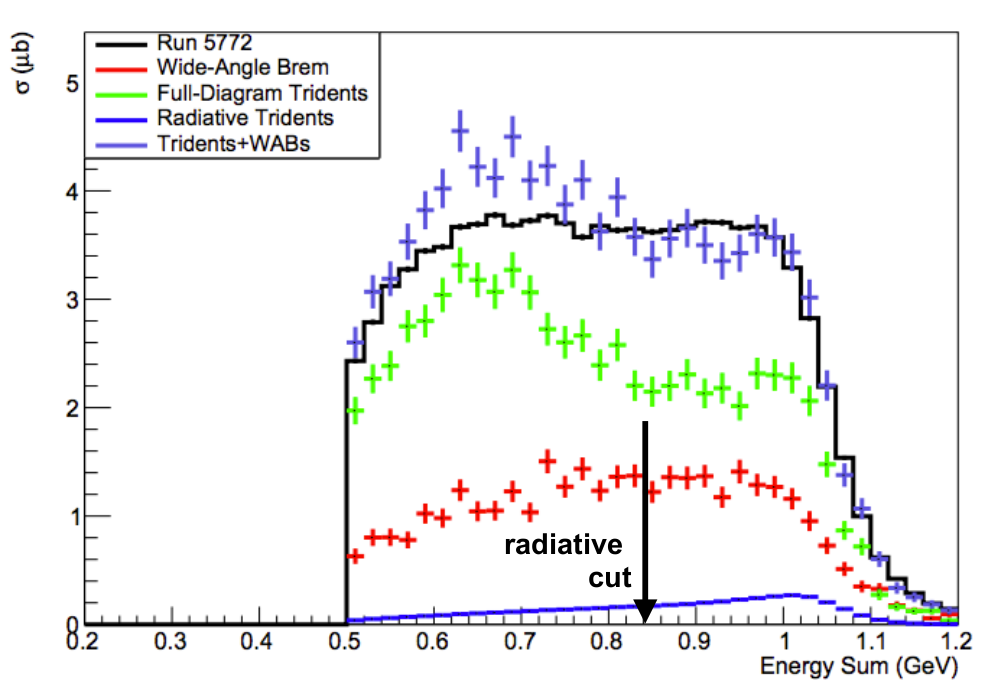
\includegraphics[width=0.55\linewidth]{figs/psum_minimal_mattg.png}
\end{figure}

\end{frame}

%------------------------------------------------

\begin{frame}
\frametitle{P Sum Comparison 2/2}
\begin{itemize}
\item Left is minimal cuts. Right is full vertexing cuts.
\end{itemize}
\begin{figure}
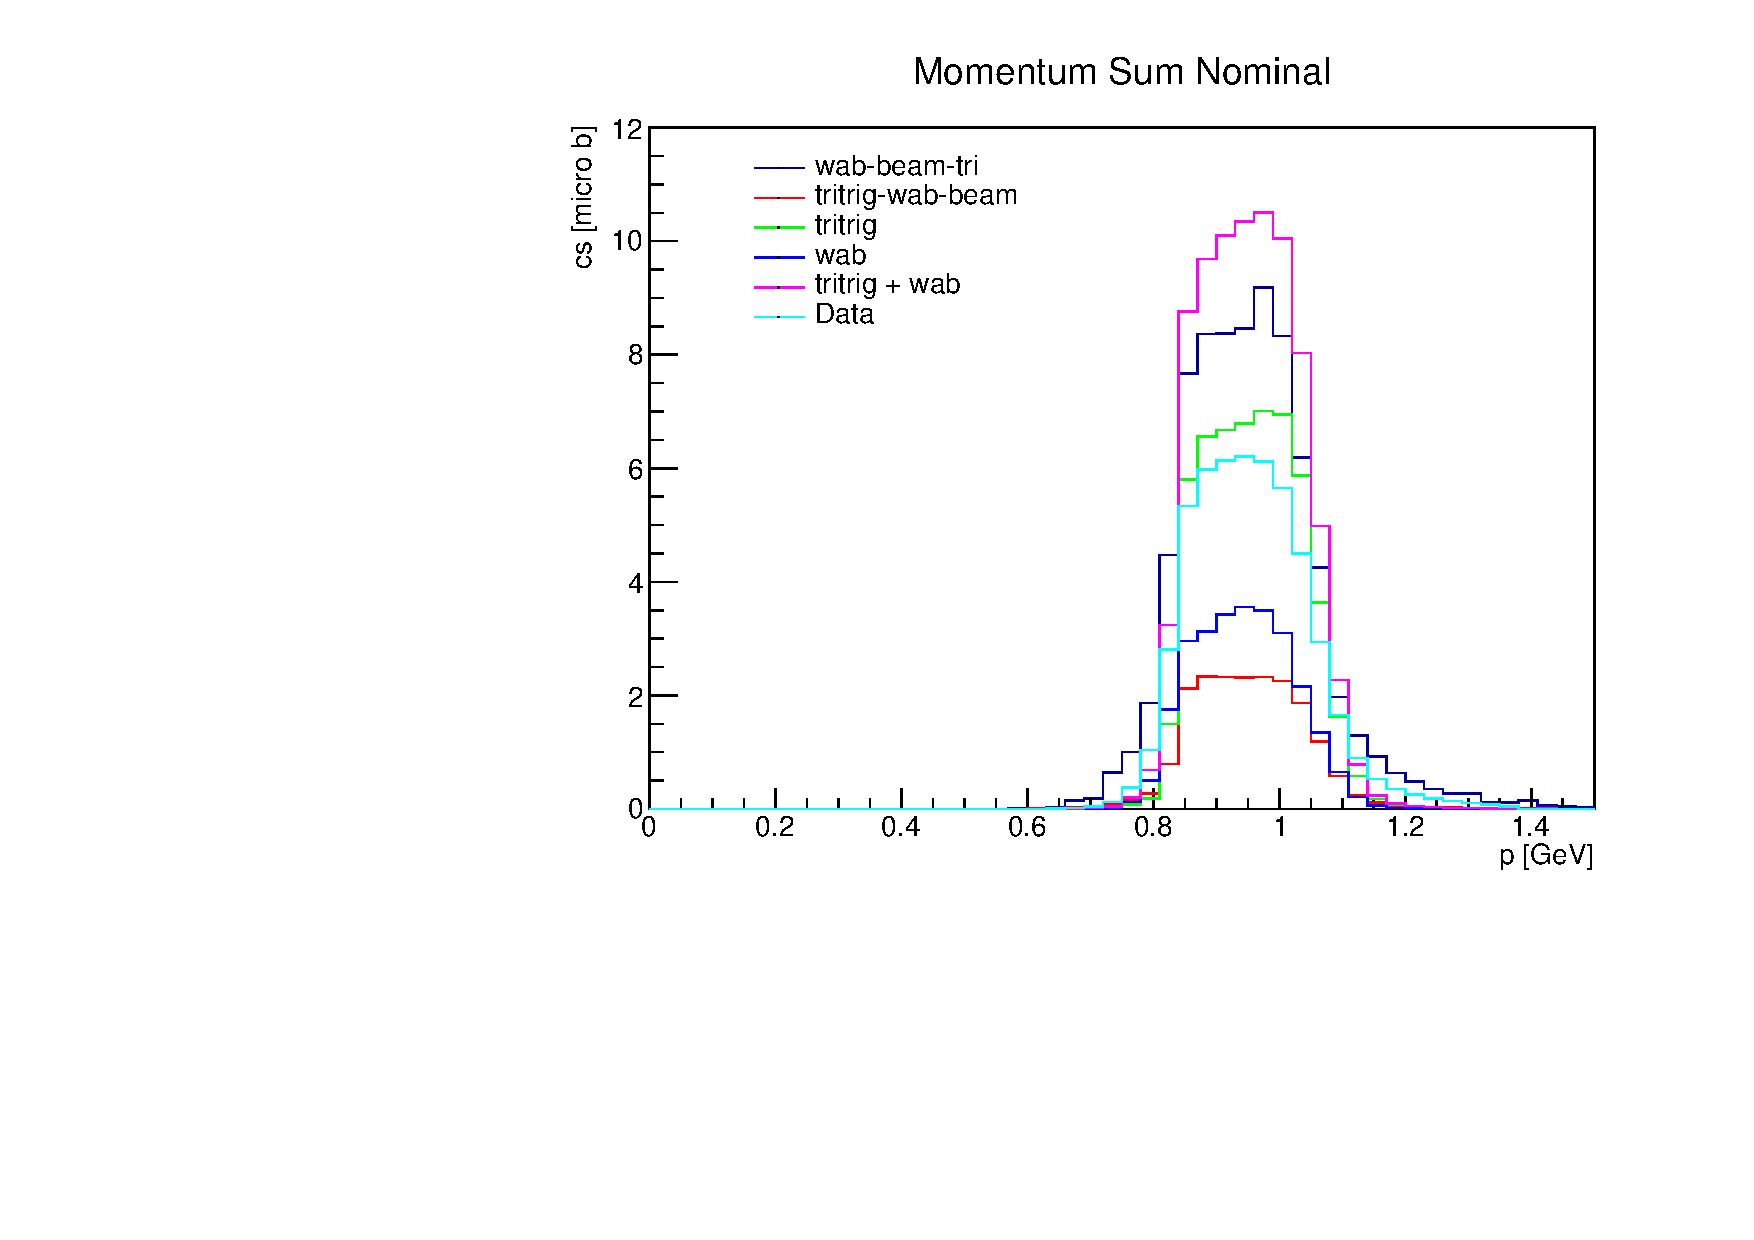
\includegraphics[width=0.55\linewidth]{figs/psum_minimal.pdf}
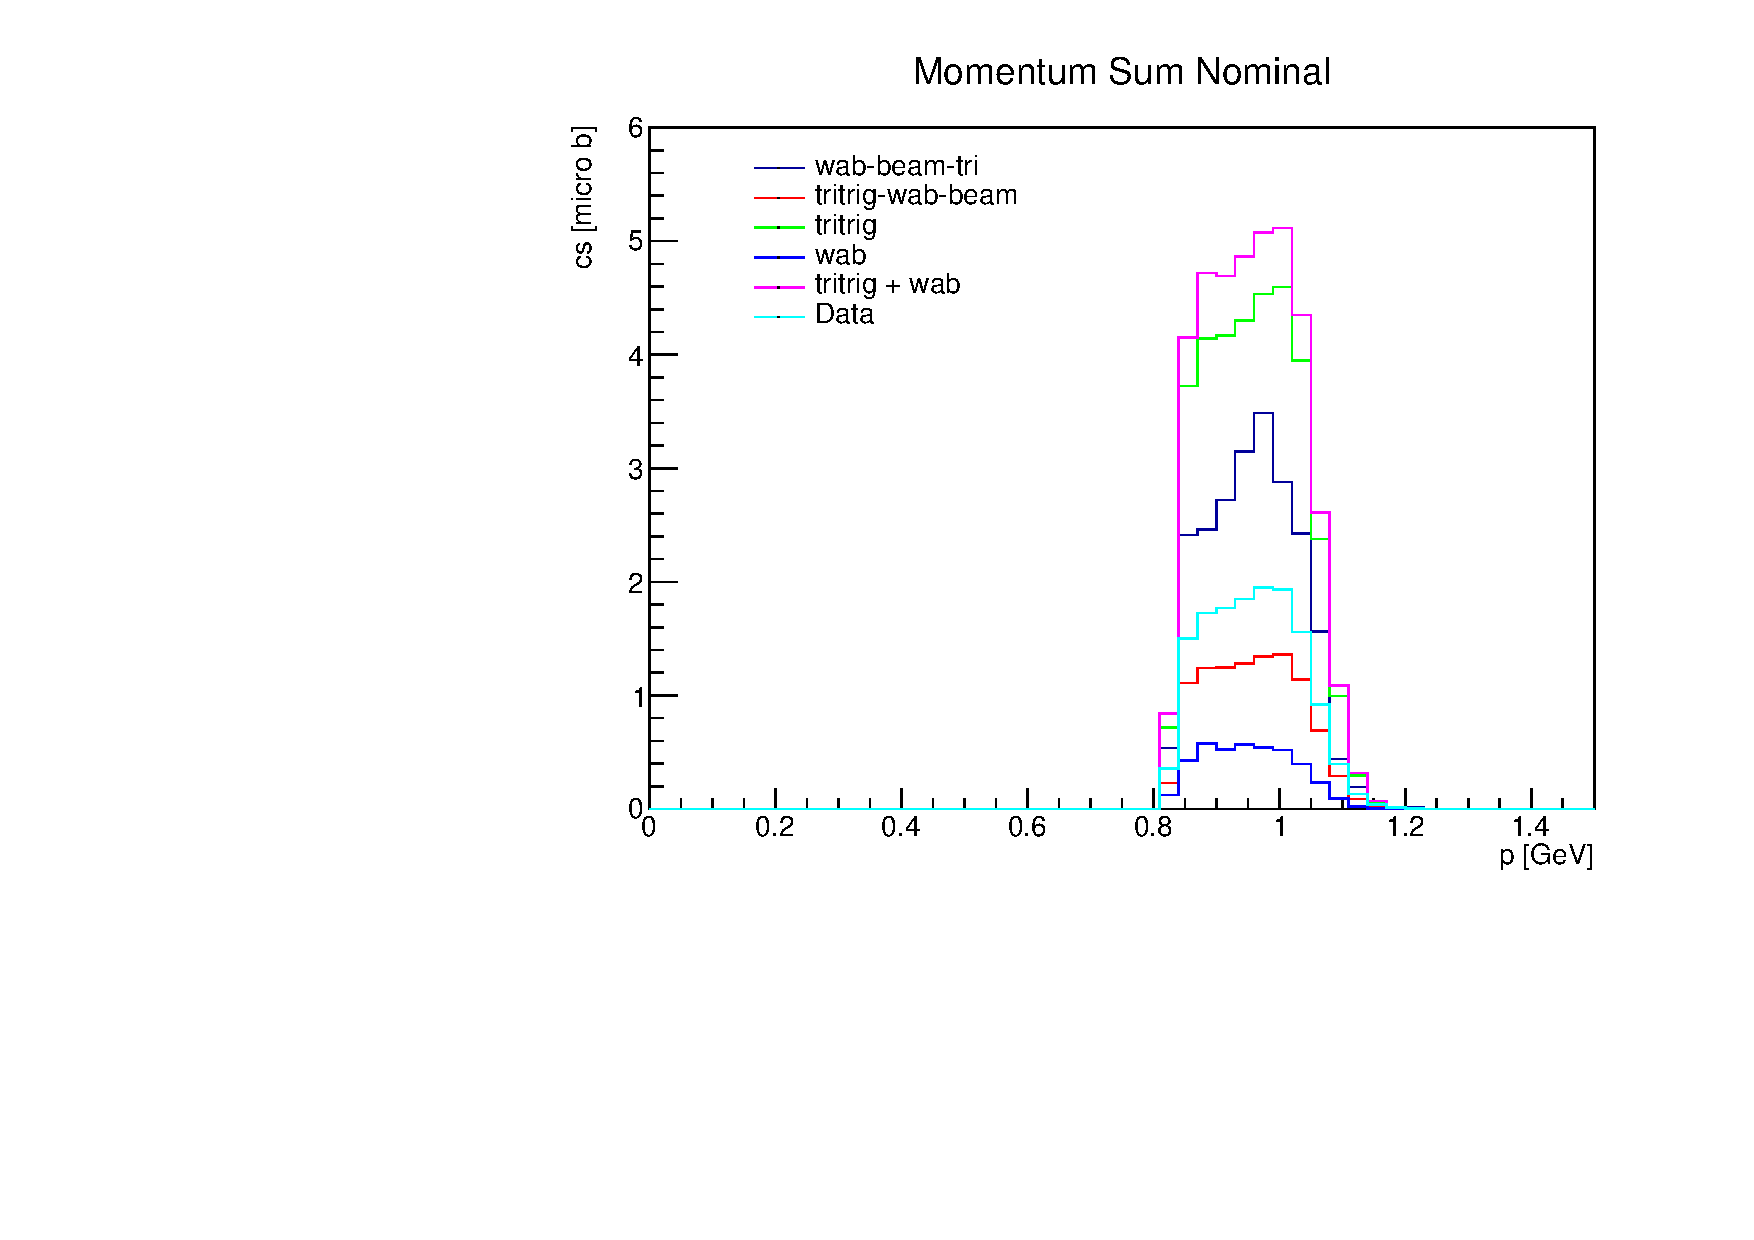
\includegraphics[width=0.55\linewidth]{figs/psum_vertexing.pdf}
\end{figure}

\end{frame}

%------------------------------------------------

\begin{frame}
\frametitle{Normalization Description}
\begin{itemize}
\item tritrig
$L=\frac{N_{gen}}{xs}*\alpha_{corr}=\frac{7,900,000}{1.3 mB}*0.78=4.74 \frac{1}{nb}$
\item wab-beam-tri
$L = t_{beam} L_{rate}=10 s \frac{1200 \frac{1}{nb}}{1.7 days}=0.0812 \frac{1}{nb}$
\item data
$L = 120 \frac{1}{nb}$
\item wabs
$L=\frac{N_{gen}}{xs}*\alpha_{corr}=\frac{1,151,800*200}{590.207 mB}*0.81=0.316 \frac{1}{nb}$
\item tritrig-wab-beam
$L=\frac{N_{gen}}{xs}*\alpha_{corr}=\frac{200,000,000}{1.3 mB}*0.78=120 \frac{1}{nb}$
\end{itemize}

\end{frame}

%------------------------------------------------

\begin{frame}
\frametitle{MC Chain Comparison}
\begin{itemize}
\item Why is the trigger rate so much lower for tritrig-wab-beam compared to tritrig?
\end{itemize}
\begin{figure}
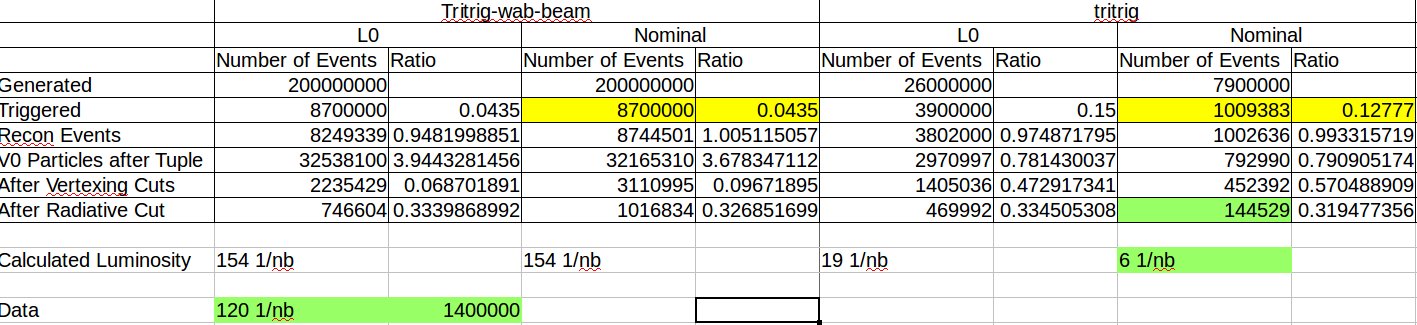
\includegraphics[width=1.0\linewidth]{figs/norm_xs.png}
\end{figure}

\end{frame}

%------------------------------------------------

\end{document} 
